\documentclass[12pt]{article}

\usepackage[utf8x]{inputenc}
\usepackage[english]{babel}

\usepackage{amssymb,amsmath,amsthm,amsfonts}
\usepackage{calc}
\usepackage{graphicx}
\usepackage{subfigure}
\usepackage{gensymb}
\usepackage{url}
\usepackage[utf8x]{inputenc}
\usepackage[T1]{fontenc}
\usepackage{amsmath}
\usepackage{graphicx}
\graphicspath{{images/}}
\usepackage{parskip}
\usepackage{fancyhdr}
\usepackage{vmargin}
\usepackage{etoolbox}
\usepackage{flafter}
\usepackage{multirow}
\patchcmd{\thebibliography}{\section*}{\section}{}{}
\setmarginsrb{3 cm}{2.5 cm}{3 cm}{2.5 cm}{1 cm}{1.5 cm}{1 cm}{1.5 cm}

\title{Prospector Sea Floor Mapping System}					
\author{SPMP}										


\makeatletter
\let\thetitle\@title
\let\theauthor\@author
\let\thedate\@date
\makeatother

\pagestyle{fancy}
\fancyhf{}
\rhead{\theauthor}
\lhead{\thetitle}
\cfoot{\thepage}

\begin{document}

%%%%%%%%%%%%%%%%%%%%%%%%%%%%%%%%%%%%%%%%%%%%%%%%%%%%%%%%%%%%%%%%%%%%%%%%%%%%%%%%%%%%%%%%%

\begin{titlepage}
	\centering
    \vspace*{0.0 cm}
    \textsc{\LARGE Software Project Management Plan (SPMP)}\\[2.0 cm]
	\textsc{\Large Software Engineering and Project}\\[0.5 cm]			
	\textsc{\large University of Adelaide}\\[0.5 cm]
	\rule{\linewidth}{0.2 mm} \\[0.4 cm]
	{ \huge \bfseries \thetitle}\\
	\rule{\linewidth}{0.2 mm} \\[1.5 cm]
	
	\begin{minipage}{0.4\textwidth}
		\begin{center} \large
			Navdeep Singh (1660360)\linebreak
			Liang Yuan (1679380)\linebreak
			Zeqi Fu (1680895)\linebreak
			Tao Zhang (1680974)\linebreak
			Lili Wu (1683229)\linebreak
			Yi Lin (1682781)\linebreak
            Yann Frizenschaf (1162562)\linebreak
			\end{center}
	\end{minipage}\\[2 cm]
	
	{\large Semester 2, 2016}\\[2 cm]
 
	\vfill
	
\end{titlepage}

\pagenumbering{roman}
\begin{table}
\begin{tabular}{ | p{0.11\textwidth}| p{0.22\textwidth}| p{0.10\textwidth}| p{0.34\textwidth}|p{0.1\textwidth}|}
\hline
\multicolumn{5}{|c|}{\textbf{Revision History}}\\
\hline
\textbf \textbf{Date} &  \textbf\textbf{Name} &  \textbf\textbf{ID} & \textbf\textbf {Updates} & \textbf\textbf{Version} \\
\hline
23th Aug & Navdeep Singh & 1660360 & Added the basic structure of draft  & 0.1\\
\hline
25th Aug & Navdeep Singh & 1660360 &Updated the project deliverables & 0.2\\
\hline
29th Aug & Lili Wu & 1683229 &Updated the definitions and glossary& 0.3\\
\hline
29th Aug&Yi Lin  &1682781  &Added the risk management plan & 0.4\\
\hline
 30th Aug&Yi Lin  &1682781 &Added the quality assurance plan & 0.5\\
\hline
 30th Aug&Yi Lin  &1682781  &Updated the risk management plan& 0.6\\ 
\hline
  30th Aug&Liang Yuan  &1679380  &Added the configuration management plan &0.7\\
\hline
 1st Sep&Yi Lin  &1682781  &Update the  quality assurance plan & 0.8\\
 \hline
 3th Sep&Liang Yuan  &1679380  & Updated the configuration management plan & 0.9\\
\hline
 4th Sep& Yann Frizenschaf &1162562   &Reviewed all the content and added suggestions on revision & 0.10\\
 \hline
 5th Aug & Lili Wu & 1683229 &Updated the assumptions and constraints& 0.11\\
\hline
5th Aug & Lili Wu & 1683229 &Updated the documentation preparation and versioning& 0.12\\
\hline
 6th Sep& Yann Frizenschaf &1162562   &Updated the process model section and fixed the format problems & 0.13\\
 \hline
  6th Sep& Yann Frizenschaf &1162562   &Updated the risk management plan & 0.14\\
 \hline
 6th Sep& Yann Frizenschaf &1162562   &Updated the milestone section & 0.14\\
 \hline
 6th Sep& Yi Lin &1682781   &Updated the revision history & 0.15\\
 \hline
 7th Sep & Yann Frizenschaf & 1162562 & Final edits & 0.16\\
\hline
 8th Sep & Yann Frizenschaf & 1162562 & Draft release & 1.0\\
\hline
12th Oct & Yi Lin & 1682781 & Updated the tables of likelihood and severity & 1.1\\
\hline
25th Oct & Yann Frizenschaf & 1162562 & Updated Sections 4 and 5 for final release & 2.0\\
\hline
\end{tabular}
\end{table} 
\pagebreak

\clearpage 

\pagebreak
\tableofcontents
\pagebreak

\pagenumbering{arabic}

\section{Introduction}

\subsection{Purpose}

The purpose of this document is to detail the Software Project Management Plan for the Prospector Seafloor Mapping System (SFM), developed for SeaFaults. It contains the details of the organisation of the project from a process and resources perspective, elicitation and mitigation of potential risks, a work plan comprising activities, milestones and proposed schedule, and plans for configuration management and quality assurance. As a whole, this document represents a detailed view of the processes and artefacts required to deliver the functionality specified in the associated Software Requirements Specification (SRS) \cite{srs}, and to prove that the aforementioned functionality has, in fact, been delivered.

\subsection{Scope}

This document defines the management plan for the software component
of the SFM system only. While hardware considerations are touched
on in some sections, the hardware to be
used has been defined and consideration of this (beyond its basic configuration and effect
on the requirements of the software system) are beyond the scope of
both this document and the project as a whole. 

\subsection{Assumptions and constraints}
\subsubsection{Assumptions}
\begin{itemize}{}
\item The specifications for the project have been provided by the client \cite{spec}.
\item The detailed requirements have been elicited in the initial stage of the project (see Section \ref{procphases}).
\item The client's representatives have knowledge of the project domain (sea floor mapping), but not necessarily of software development or implementation.
\item The project team have knowledge of software development and implementation, but not necessarily of the project domain.
\item The process model used during the project is to be selected and followed by the project team (client has no strong preference).
\item The client expects the project's quality assurance processes to be as close as feasible to current best practices for software development.
\end{itemize}

\subsubsection{Constraints}
\begin{itemize}{}
\item Team members have varying levels of skill in writing both Java code and English language documents. 
\item The accuracy of the provided sensor and actuator hardware is likely to fall short of what is desired to obtain the requisite mapping accuracy.
\item The project has a firm deadline for delivery, and the resourcing (number of team members) is fixed and will not change for the duration of the project.
\item The client has specified limits for external code (libraries) which may be used in the software delivered; this has been capped at 10%.
\end{itemize}

\subsection{Project deliverables}\label{deliverables}
The major deliverables for the project have been defined by the client (SeaFaults) and are enumerated below, and due dates for each are specified in Section \ref{milestones}:
\begin{enumerate}{}
\item{\textbf{Software Requirements Specification:}} Defines the requirements for the software component of the SFM system, as well as detailing the assumptions inherent in and constraints upon those requirements

\item{\textbf{Software Project Management Plan:}} Defines the technical and managerial Processes necessary for the development and delivery of the SFM system (this document).

\item{\textbf{Software Design Document:}} Describes the design goals of the SFM system, as well as trade-offs made between design goals, software control implementations and systematic constraints.

\item{\textbf{Testing Report:}} Contains the details of all planned an conducted tests of the delivered system, and the outcomes of those tests. Includes both functional tests (system demonstration) and automated tests (i.e. unit tests).

\item{\textbf{User Manual:}} A detailed set of instructions for the SFM system's end user(s). Includes all instructions necessary to perform all delivered functions of the system, and assumes the reader has basic knowledge of computer/GUI use, but no detailed knowledge of the inner workings of the system.

\item{\textbf{Milestone Software Demonstration 1:}} A demonstration of the functionality milestones negotiated with the client to be delivered by an agreed date for milestone 1.

\item{\textbf{Milestone Software Demonstration 2:}} A demonstration of the functionality milestones negotiated with the client to be delivered by an agreed date for milestone 2.

\item\textbf{{As-built Software Demonstration:}} The major testing event required for the SFM project. Demonstrates to the client all features of the system as-built in a single demonstration session.

\end{enumerate}

\subsection{Evolution of the plan}
As per the agile project management philosophy detailed in Section \ref{procmodel}, the details of the plan contained within this document are subject to evolution and change as requirements change, hitherto unknown challenges are discovered, and unforeseen changes of circumstances arise with respect to resourcing, scheduling, tooling or functional constraints. These changes will be captured in the agile process model where possible, and made evident to the client in a prompt and transparent manner.


\section{Project organisation}\label{funcrec}
\subsection{Process model}\label{procmodel}

For the purposes of this project, an agile project management methodology has been chosen. Several key aspects of the SFM project align closely with the strengths of the agile process model, including:
\begin{itemize}{}
\item Rapid development cycle favouring incremental changes and delivery
\item Frequent customer involvement and continuous feedback on developed features
\item Small, focused team
\item Focus on both functional and automated testing to validate project outcomes
\end{itemize}

Key details in this section regarding the agile approach and its implementation are informed by \cite{sommerville}.

\subsubsection{Agile approach}
The general philosophy of the agile project management approach requires work to be divided into work items achievable by a single team member within a specified work period, called a sprint. Sprints are typically short (for the purposes of this project, one week in duration) and generally aim to deliver a functional system in some form. 

Work items are added to a backlog and prioritised in order of importance and/or urgency. The expected effort required to completed each item is estimated by the team. If an item cannot be estimated, it is underspecified, and if it is estimated to take longer than one sprint, it must be broken down into smaller items.
At the start of each sprint, work items (also sometimes referred to as "stories") are added to the sprint in priority order until the team's capacity is reached for the sprint period, and the sprint begins. Team members work on assigned items until the sprint is complete.

Work items can be classified as subsets of major features or "epics", and a feature can be considered to be complete when all associated work items are completed. This allows a line to be drawn between work items and deliverable features, and aids in estimation of remaining time required to complete a feature (see Section \ref{agilerisk}). Sprints are organised into releases, usually corresponding to a major milestone delivery or demonstration (see Figure \ref{fig:agile}). The release process for this project is explained in detail in Section \ref{releases}.

The backlog is an evolving list of items to be completed, which may grow as work is discovered during the development process, and shrink as items are completed. Any team member can create work items, but only the Project Liaison may priorities them, and only the Scrum Master may add or remove items from a sprint based on priority. These roles are explained in more detail below.

\begin{figure}[h!]
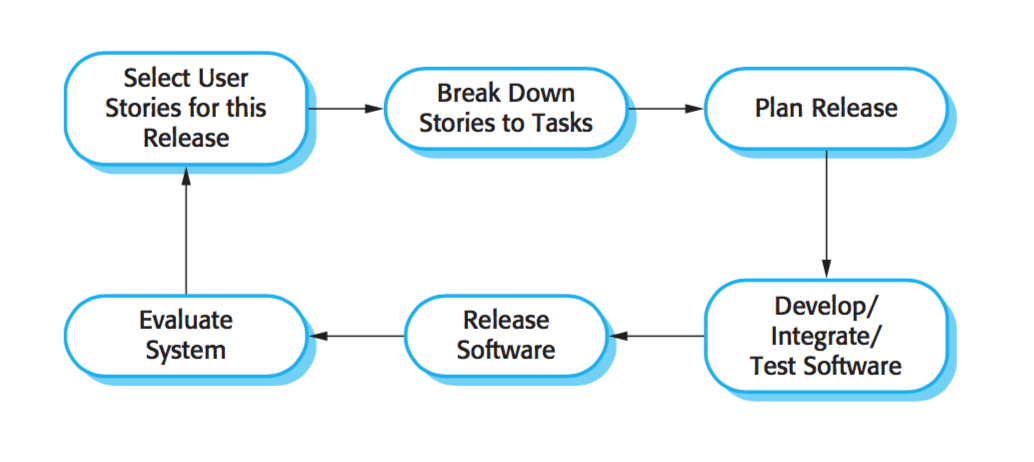
\includegraphics[width=\textwidth]{The_extreme_programming_release_cycle.png}
\caption{Overview of the agile release cycle \cite{sommerville}}
  \label{fig:agile}
\end{figure}

\subsubsection{Roles}\label{procroles}
Apart from the development team itself, the following roles are defined in the context of agile project management:
\begin{description}
\item{\textbf{Project Liaison:}} While a member of the team, the Project Liaison represents the customer's interests. In this capacity, it is the role of the Project Liaison to determine the priority of work items and ensure they are suitably specified and in line with the project requirements as detailed in the SRS.
\item{\textbf{Scrum Master:}} The scrum master's role is to ensure the team's workload is correctly distributed, the team is free from external distractions, and informs the Project Liaison if the backlog is not organised or specified to the team's satisfaction.
\end{description}
Strictly speaking, the Project Liaison and scrum master should not be the same person, and both should be separate from the development team where possible. In very small projects, however, such separation may not be possible due to resourcing constraints. 
For the purpose of this project, the Project Liaison and scrum master roles are fulfilled by the same person under the umbrella term project manager.

\subsubsection{Phases}\label{procphases}
While agile development is fundamentally incremental, it can be beneficial to divide the project into phases to reflect the varying process requirements at different stages of the project. The phases defined for this project are as follows:
\begin{description}
\item{\textbf{Requirements Elicitation:}} Several meetings are held with the client in order to flesh out requirements and clarify any ambiguities in the original broad specification. It is possible that no formal sprints are conducted during this time, but high-level software architecture is designed and preliminary hardware tests are performed to determine project constraints.
\item{\textbf{Rapid Prototyping:}} Formal sprints commence in order to deliver an early prototype of user-facing functionality. This phase serves to give an early concrete form to the outcomes of the requirements elicitation and give opportunity for client feedback prior to the main development phase. This prototype represents the first informal release of software for the project.
\item{\textbf{Product Development:}} Based on the outcomes of the requirements elicitation and rapid prototyping phases, formal development of the main software product commences. Releases are scheduled to coincide with deliverable milestones, and sprints are scheduled within release periods.
\item{\textbf{Post-release:}} After the release of the final version of the software, there may be a further requirement to finalise as-built documentation and/or testing reports. Formal sprints may not be necessary in this phase.
\end{description}

Note that as per the agile project management approach, there is no standalone testing phase, as comprehensive feature and regression testing is to occur with each incremental release. The specific start and finish dates for these phases are detailed in Section \ref{schedule}.

\subsubsection{Risks and Reporting}\label{agilerisk}
The agile project management approach is not without risk; unlike in a more traditional waterfall-based approach, there is no intrinsic method for tracing a schedule's critical path. However, various reporting methods are available to project managers in order to satisfy the need to report progress to the client. The primary reporting metric used in this project will be burndown charts (see Figure \ref{fig:burndown}), which report remaining effort required for completion of all work items on a per-sprint and per-release basis. 

Estimation represents a significant challenge in the agile process, and therefore requires careful consideration. Often, work item effort is estimated in "points" rather hours in order to ensure that the estimate is a measure of complexity or difficulty of the task rather than the time it will require. This is because different tasks may require different amounts of time to complete the same item, and using points as an abstract measure helps normalise this discrepancy across the team in each sprint \cite{cohn}. Sprint and/or release progress can be measured using one of two metrics: work items completed or story points completed, depending on the level of granularity required.

\subsubsection{Tools}
Several tools are available from major vendors for tracking agile software projects. The three main contenders considered for use in this project included Jira (Atlassian), Visual Studio Team Services (Microsoft) and YouTrack (JetBrains), all of which have feature sets adequate for the requirements of this project. Of these, only YouTrack offered a free, in-cloud option for the required number of users (7). As such, YouTrack was selected as the project tracking tool of choice.

\begin{figure}[h!]
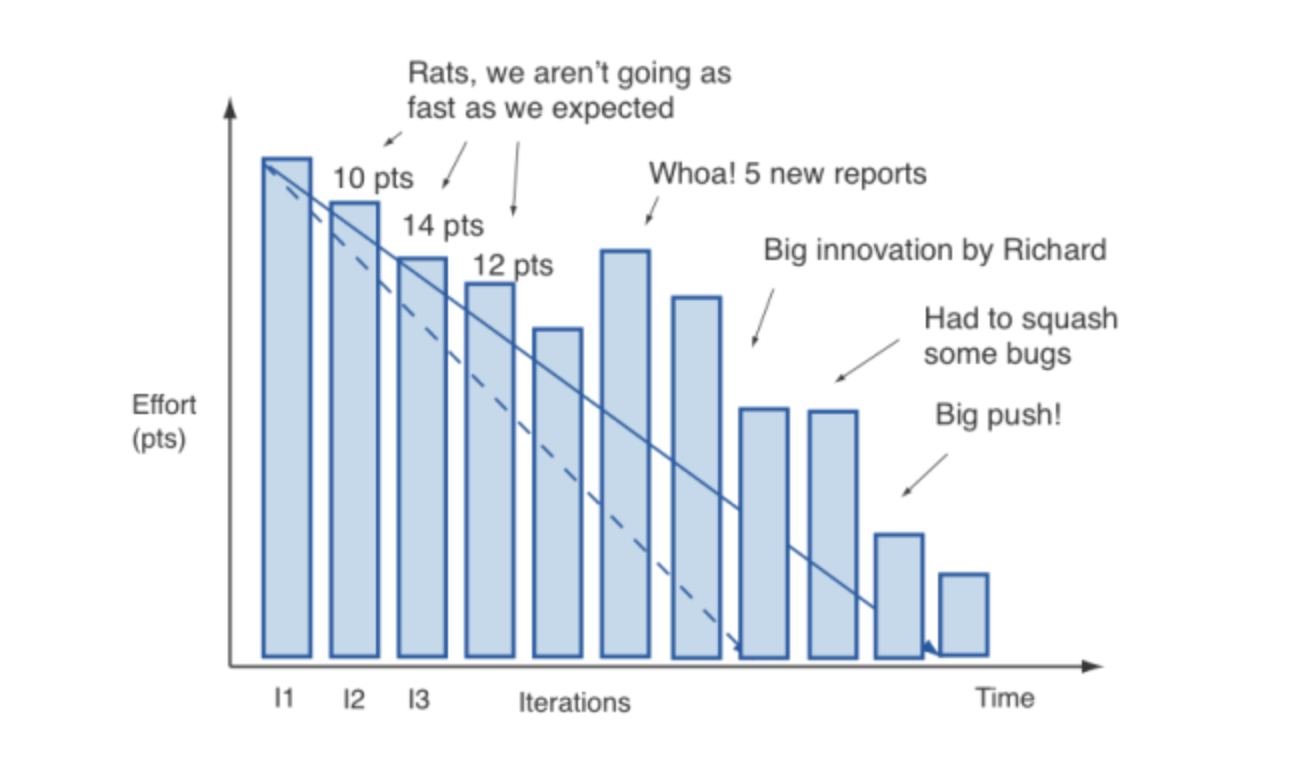
\includegraphics[width=\textwidth]{A_burndown_chart_example.png}
\caption{An annotated example of a typical burndown chart \cite{rasmusson}}
  \label{fig:burndown}
\end{figure}

\subsection{Roles and responsibilities}\label{roles}
In order to facilitate working in parallel, the software development work required to complete the project has been divided into three main functional areas: \textbf{movement} (controlling the motion of the robot in response to operator commands and sensor input, as well as estimating robot position in real-time), \textbf{sensors} (gathering and synthesising sensor input for use by the movement and mapping systems), and \textbf{mapping} (constructing a map of the survey in real-time based on sensor input and estimated position). The breakdown of the team in functional areas, as well as project management roles, is detailed below:

\begin{description}
\item[{Project Manager:}]Yann Frizenschaf \\
The role of the project manager is to oversee scheduling and resource allocation, as well as to perform the Project Liaison and Scrum Master roles as detailed in Section \ref{procroles}.

\item[{Assistant Project Manager:}]Tao Zhang \\
The role of the assistant project manager is to support the project manager in facilitating scheduling and work delegation, and assume the project manager's responsibilities if the project manager is for any reason unable to do so.

\item[{QA Manager:}]Lili Wu \\
The quality assurance manager is responsible for ensuring test artefacts are developed and testing activities proceed as per the quality assurance plan (see Section \ref{QA}).

\item[{Documentation Manager:}]Navdeep Singh \\
The documentation manager is to ensure that the project documentation is delivered on time and to the required quality standard, coordinating team members' contributions to the documentation, and making sure versioning of documents is correct.

\subsubsection{Functional teams}

\item[{Movement:}]Tao Zhang, Yi Lin

\item [{Sensors:}]Lili Wu, Navdeep Singh, Liang Yuan

\item[{Mapping:}]Zeqi Fu, Yann Frizenschaf

\end{description}

\section{Risk Management Plan}
Risks to successful and timely completion of the project are detailed in Table \ref{table:risk}, including the severity and likelihood of each risk scenario.  In Table\ref{table:Severity} , explains the severity and likelihood.  In Table \ref{table:mitigation}, strategies for mitigating the identified risks are detailed. The common identifier across the two tables is the risk ID. 

There are six main risk categories. These are technology risks, human resources risks, organisational risks, tooling risks, requirements risks, and estimation risks. In Tables \ref{table:risk} and \ref{table:mitigation}, R01 to R03 are technology risks, R04 to R05 are human resource risks, R06 to R07 are organisational risks, R08 to R10 are tooling risks, R11 to R12 are requirements risks, and R13 is an estimation risk.

\begin{table}
\begin{tabular}{ | p{0.15\textwidth} | p{0.55\textwidth}| p{0.15\textwidth} |p{0.15\textwidth}|}
\hline
\textbf{Risk ID} &  \textbf{Description} &  \textbf {Severity} & \textbf{Likelihood} \\
\hline
R01 & Software defects cause test failure & Medium & High\\
\hline
R02 & Team members leave the team &  Medium & Low\\
\hline
R03 & Data loss & High & Medium\\
\hline
R04 & Underestimation of required effort & Medium & Medium\\
\hline
R05 & Communication difficulties between team members & Medium & Low\\
\hline
R06 & Tasks are not allocated reasonably & Medium & Medium \\
\hline
R07 & Unexpected changes to requirements & Medium & High\\
\hline
R08 & Hardware damage to robot & High & Medium\\
\hline
R09 & Failure of robot remote communication & High & High\\
\hline
R10& Loss of robot hardware &High &Medium\\
\hline
R11 & Schedule slippage & High & Medium\\
\hline
R12 & Adding new requirements & Medium &Medium\\
\hline
R13 & Estimated testing time not sufficient to complete test activities &High &High\\
\hline 

\end{tabular}
\caption{Identified risks}
\label{table:risk}
\end{table} 

\begin{table}
\centering
\begin{tabular}{ | p{0.15\textwidth} | p{0.55\textwidth}|}
\hline
\textbf{Level} & \textbf{Description} \\
\hline
High & Highly likely to result in project failure\\
\hline
Medium & Failure to meet core goals\\ 
\hline
Low & Failure to meet extension goals\\
\hline
\end{tabular}
\caption{Severity identification}
\label{table:Severity}
\end{table}

\begin{table}
\centering
\begin{tabular}{ | p{0.15\textwidth} | p{0.55\textwidth}|}
\hline
\textbf{Level} & \textbf{Description} \\
\hline
High & >85\% percent chance of occurrence\\
\hline
Medium & >40\% percent chance of occurrence\\ 
\hline
Low & <40\% percent chance of occurrence\\
\hline
\end{tabular}
\caption{Likelihood identification}
\label{table:Likelihood}
\end{table}

\begin{table}
\begin{tabular}{ | p{0.15\textwidth} | p{0.43\textwidth}| p{0.49\textwidth} |}
\hline
\textbf{Risk ID} & \textbf{Risk Cause} & \textbf{Risk minimisation/mitigation plan}\\
\hline
R01 & Insufficient testing & Implement comprehensive test plan \\
\hline
R02 & Members withdraw from the course & Implement role-based redundancy\\
\hline
R03 & Computer hardware failure & Distributed backups\\
\hline
R04 & Differences in skills and experience across team & Arrange for team members to complete tasks that match up with their individual skills \\
\hline
R05 & Team members' native languages are different & Important decisions confirmed in written form\\  
\hline
R06 & The working plan is not suitable for an individual & Ensure flexibility of task assignment as per agile process model \\
\hline
R07 & Client requirements change or work is discovered & Perform regular requirements review\\
\hline
R08 & Inadequate safety measures during testing & Ensure safety measures are reflected in functional test plan\\
\hline
R09 & Primary wireless communication method is unstable & Ensure backup communication plan is tested and software fail-safes are implemented\\
\hline
R10 & Insecure storage & Ensure robot is stored in secure locker when not in use\\
\hline
R11 & Inadequate estimation process & Adapt estimation process as per agile process model \\
\hline
R12 & Discovered work, unexpected bugs, new requirements  & Negotiate feature and schedule change with client at earliest opportunity\\
\hline
R13 & Schedule slippage & Prioritise testing of existing features over new feature addition\\
\hline
\end{tabular}
\caption{Risk causes and minimisation/mitigation}
\label{table:mitigation}
\end{table} 

\section{Work plan}
The work plan detailed below represents the preliminary plan for the scheduling, and execution of the project works.

\subsection{Work Activities}\label{schedule}

The start and finish dates for the project phases introduced in Section \ref{procphases} are detailed in Table \ref{table:schedule}.

\begin{table}
\begin{tabular}{ | p{0.15\textwidth} | p{0.55\textwidth}| p{0.15\textwidth} |p{0.15\textwidth}|}
\hline
\textbf \textbf{ID } &  \textbf\textbf{ Project phase } &  \textbf\textbf {Start date } & \textbf\textbf{Finish date } \\
\hline
1 & Requirements elicitation & 09/08/2016 & 22/08/2016 \\
\hline
2 & Rapid prototyping: & 22/08/2016 & 13/09/2016 \\
\hline
3 & Product development & 13/09/2016 & 30/10/2016 \\
\hline
4 & Post-release & 30/10/2016 & 01/11/2016  \\
\hline
\end{tabular}
\caption{Schedule of major project phases}
\label{table:schedule}
\end{table} 

\subsection{Milestones and release plan}\label{milestones}
The delivery dates for project artefacts and key milestones are detailed in Table \ref{table:milestones}. At each of the two interim milestones, at least one major feature will be demonstrated in order to demonstrate development progress to  the customer. The major features to be completed in each release, broken down by functional area, are detailed in Figure \ref{fig:features}.

As can be seen in Figure \ref{fig:features}, the number of features completed in later releases is lower than the number completed in earlier releases. This is due to the complexity of developed features increasing toward the end of the project (i.e. fully autonomous operation), relative to the early features.

The features to be included in each release are based on the judgment of the team, and to be negotiated with the client.

\begin{table}
\begin{tabular}{ | p{0.75\textwidth} | p{0.25\textwidth} |p{0.0\textwidth}|}
\hline
\textbf{Deliverable/Milestone } & \textbf{Due Date} \\
\hline
Software Requirements Specification & 01/11/2016  \\
\hline
Software Project Management Plan &  01/11/2016   \\
\hline
Software Design Document &  01/11/2016  \\
\hline
Testing Report &  01/11/2016  \\
\hline
User Manual &  01/11/2016  \\
\hline
Milestone Software Demonstration 1 &  13/09/2016  \\
\hline
Milestone Software Demonstration 2 &  04/10/2016  \\
\hline
As-built Software Demonstration &  01/11/2016  \\
\hline
\end{tabular}
\caption{Delivery dates for project artefacts and milestones}
\label{table:milestones}
\end{table}

\begin{figure}[htp!]
\centering\includegraphics[width=\textwidth]{features.png}
\caption{Feature breakdown by release}
  \label{fig:features}
\end{figure}

\subsection{Schedule and resource allocation }
The estimated workload for the team as a whole is established once  for each phase of the project, at the beginning of the phase. Additionally, adjustments in the schedule will be made for each of the team members on a per-release and per-sprint basis, depending on the workload for the given period of time. The goal for each sprint is to complete the allocated work as a team, so tasks can be reassigned to team members who finish their assigned tasks early.

In general, software development works will be divided by functional area as detailed in Section \ref{roles}, and documentation work will be divided by document section. However, in some cases team members may be required to assist colleagues outside of their functional team, as per the agile approach, in order to achieve sprint/release completion.

In some cases, it may be necessary to push unfinished tasks to a later sprint if the required effort was underestimated. Similarly, it may be possible to bring tasks forward if the total sprint effort was initially overestimated. In this way, the inherent error in the agile estimation process is intended to even out \cite{sommerville}. If effort is found to be consistently under-estimated, however, the team will be required to re-calibrate the estimation process by intentionally adding some overhead to estimates going forward.

\section{Supporting plans}\label{funcrec}
\subsection{Configuration management}
Configuration management serves to ensure that the current design and build state of the project is known. It allows access to a historical record of project state relevant for  both project management and development activities. The benefits of a comprehensive configuration management plan include [4]:
\begin{itemize}
\item Maintaining the integrity of the project.
\item Tracking the changes during development.
\item Providing an ability to trace the process that from requirement to product.
\item Reducing the cost of maintaining project.
\item Providing a stable environment for software development.
\end{itemize}

\subsubsection{Software configuration management plan}

The architecture of the Prospector software project is broken down into hierarchically-arranged functional areas as listed in Table \ref{table:architecture}. Each of these functional areas is implemented as a Java package in the project structure, and may be the child of a parent package, or a root package. In this way, functional separation of concerns is achieved and parallel development is enabled; each functional area can be treated as a black box by other functional areas, provided appropriate interfaces are defined.

\begin{table}
\begin{tabular}{ | p{0.15\textwidth} | p{0.55\textwidth}| p{0.15\textwidth} |p{0.15\textwidth}|}
\hline
\textbf{Functional area} & \textbf{Description} &  \textbf{Package} &  \textbf{Parent package}\\
\hline
Prospector & Root package & prospector & - \\
\hline
Movement & Motor control, position estimation & movement & prospector \\
\hline
Vision & Sensor input synthesis & vision & prospector \\
\hline
Mapping & Map generation & mapping & prospector \\
\hline
Operations GUI & Operator HMI & opsgui & prospector \\
\hline
Data IO & Database and file management & dataio & prospector \\
\hline
File operations & Map file saving and loading & fileops & dataio \\
\hline
Database operations & Map database management & databaseops & dataio \\
\hline
Unit tests & Automated software testing & test & prospectortest \\
\hline
\end{tabular}
\caption{Software architecture configuration}
\label{table:architecture}
\end{table}

\subsubsection{Version control}
Version control during all project phases is supported by the Git VCS (version control system). While Git is not a complete configuration management solution in and of itself, it enables tracking of software development history and tagging of snapshots in the development cycle, which complements the release management plan detailed in Section \ref{releases}.

The repository consists of two major subdirectories \textit{docs} and \textit{source}. The \textit{docs} directory contains all the documentation relevant to the project, and is divided into \textit{draft} and \textit{final} subdirectories, which contain in-progress and ready-for release documents, respectively. The \textit{source} directory contains all of the source code for the project.

\subsubsection{Software releases}\label{releases}
Each software release represents a working version of the software system which is functional and feature-complete with respect to the requirements of the corresponding milestone. Each release will be accompanied by suitable set of release notes detailing the relevant major features and/or bug fixes pertinent to the release. The software itself will be provided as a pre-built executable file (or files), as well as an archive of the source code and instructions for build the software from the source using the specified build tools (ANT and MAKE).

Releases are created by tagging specific revisions in the Git VCS repository, meaning a release can be uniquely identified as a snapshot in the development history of the software.

In general, the Git repository will follow a common branching model expressed eloquently by \cite{driessen}. There are two main branches, called \textit{master} and \textit{develop}. All ongoing/incremental development work will be performed on \textit{develop}, and only when the software on that branch is ready for a release will all its revisions be merged to \textit{master}. The revision which is merged will be tagged as a release and built against the automated test suite (see Section \ref{QA}). This branching model is shown in Figure \ref{fig:branches}.

\begin{figure}[h!]
\centering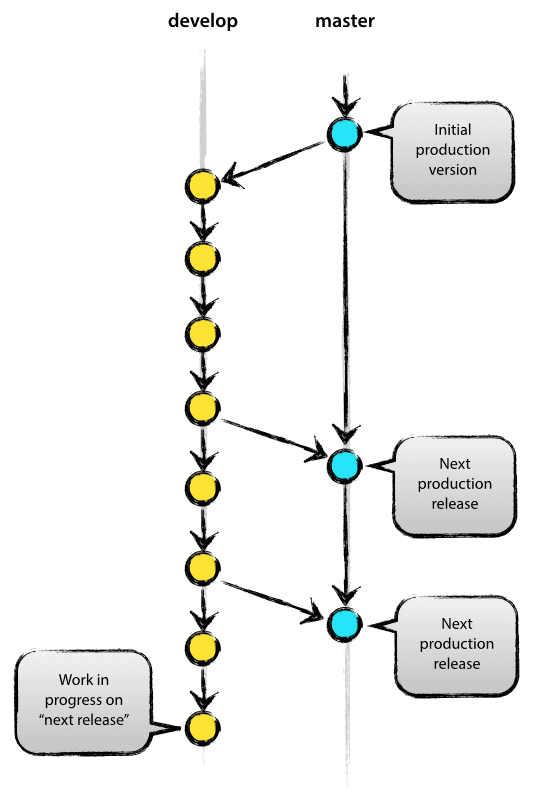
\includegraphics[width=7cm]{branches.png}
\caption{The proposed branching model \cite{driessen}}
  \label{fig:branches}
\end{figure}


\subsection{Documentation plan}
There are a number of documents that will be produced during the developing process of the project; these are listed below. Note that the requirements for the content of these documents are discussed in Section \ref{deliverables}.

\begin{enumerate}{}
\item{Software Requirements Specification} 

\item{Software Project Management Plan} 

\item{Software Design Document} 

\item{Testing Report} 

\item{User Manual} 

\end{enumerate}

\subsubsection{Documentation preparation and versioning}

Each document has a unique name, and a version number to be updated with each official revision/release (beginning with 0.1 for incremental versions and with round numbers like 1.0 for released versions). While documents are under development prior to and between releases to the client, modifications and individual contributions will be tracked via the Git VCS.

Software releases are indicated by named tags on the \textit{master} branch, one for each release, prefixed by the \textit{release} string (i.e. \textit{release-milestone-1}, \textit{release-final}. 

\subsection{Quality assurance plan}\label{QA}

Quality assurance (QA) has very important role in the Prospector SFM project. The main goals of the quality assurance plan are as follows:

\begin{itemize}{}
\item Provide the ability to quantitatively verify that the project satisfies the elicited client requirements
\item Ensure that the delivered software meets a reasonable level of quality
\item Provide the ability find and remove defects during the development phase of the project
\item Ensure that the delivered documents accurately describe the delivered software and relevant processes
\end{itemize}

\subsubsection{Software quality}
Software quality will be assured in the following ways:
\begin{description}
\item{\textbf{Unit tests:}} Fine-grained automated tests which are run as part of the software build process. Each self-contained, nontrivial software function which returns a value or alters internal state should have an accompanying unit test to ensure the output or altered state matches the provided input. Software with failing unit tests may not be released, and should not be checked in to the VCS where avoidable. Unit testing is the responsibility of each team member when developing self-contained software classes and methods.
\item{\textbf{Functional tests:}} High-level tests which demonstrate user-facing features of the software in order to quantifiable prove that the associated requirements have been met and the software is suitably defect-free. Developed by the project team under the guidance of the QA manager

\item{\textbf{System tests:}} These tests serve to ensure all the separate components of the system can work well together in an integrated fashion
\item{\textbf{Load tests:}} By subjecting the system to more trying conditions than may be found in a production environment (i.e. long operational periods, highly complex terrain), defects can be uncovered more thoroughly.

\end{description}

\subsubsection{Activities}  
The major QA activities (apart from software testing) which will be performed during the course of the project are listed below:
\begin{description}
\item{\textbf{Requirements review:}} This bulk of this activity takes place in the requirements elicitation phase of the project (see Section \ref{procphases}), but becomes an ongoing background process thereafter to ensure that development work is not proceeding tangentially to the core project requirements. This activity will be conducted by the entire project team under the guidance of the project manager.
\item{\textbf{Management review:}}This is an ongoing activity to be conducted by the project manager.  An overall view of the schedule should be maintained at least at the end of each sprint. In the case of schedule slippage, and modifications to scheduling or requirements should be negotiated with the client by the project manager on behalf of the team. The purpose of this activity is to ensure the client's expectations are in line with the likely project outcomes and delivery dates, and schedule slippage can be minimised where possible.
\item{\textbf{Code review:}}Code reviews will be conducted within functional teams on a per-sprint basis. At the end of each sprint, each team member who has contributed code changes to the software repository must ensure that the changes have been reviewed by another member of their functional team, and any feedback has been incorporated. In case of a dispute over coding style or content, a third member of the project team should serve as the tie-breaker.
\item{\textbf{Document review:}}Each document will be reviewed at least once by every contributing member of the team prior to client release. Client feedback on draft releases will be incorporated by a relevant team member, and the changes will be reviewed by at least one other team member for completeness and correctness prior to re-release.
\item{\textbf{Test review:}}All functional tests should be reviewed by both the QA manager and the functional team relevant to the functional area under test. Where possible, the high-level requirements for the outcomes of functional tests should be reviewed by a client representative. 
\end{description}


\section{Glossary}\label{glossary}

\begin{description}
\item [{GUI}] Graphical User Interface 
\item [{HMI}] Human-Machine Interface 
\item [{LeJOS}] The Lego Java Operating System 
\item [{SFM}] Sea Floor Mapping 
\item [{SRS}] Software Requirements Specification 
\item [{SPMP}] Software Project Management Plan
\item [{SDD}] Software Design Document 
\item [{VCS}] Version Control System 
\item[{QA}] Quality Assurance


\end{description}



\begin{thebibliography}{1}

\bibitem{cohn} Cohn, M 2014. \textit{The Main Benefit of Story Points}, viewed 6 September 2016, <https://www.mountaingoatsoftware.com/blog/the-main-benefit-of-story-points>
      
\bibitem{driessen} Driessen, V 2010. \textit{A successful Git branching model}, viewed 6 September 2016, <http://nvie.com/posts/a-successful-git-branching-model/>

\bibitem{spec} Milanese, D and Weerasinghe, A 2016. \textit{Software Engineering and Project - SeaFaults Mapping Robot}. Project specification version 1.0

\bibitem{srs} Prospector Team 2016. \textit{Software Requirements Specification: Prospector Seafloor Mapping System}. Version 2.0.
  
\bibitem{sommerville} Sommerville, I 2011. \textit{Software Engineering}, 9th Edition, Addison-Wesley, Boston
   
\bibitem{rasmusson} Rasmusson, J 2016. \textit{Agile in a Nutshell}, viewed 5 September 2016, <http://www.agilenutshell.com/burndown>
   

      
      

  \end{thebibliography}
\end{document}
